\documentclass[12pt, a4paper]{article}

\usepackage[czech]{babel}
\usepackage{lmodern}
\usepackage[utf8]{inputenc}
\usepackage[T1]{fontenc}
\usepackage[pdftex]{graphicx}
\usepackage{amsmath, amssymb}
\usepackage[hidelinks,unicode]{hyperref}
\usepackage{float}
\usepackage{listings}
\usepackage{tikz}
\usepackage{xcolor}
\usepackage{tabularx}
\usepackage[final]{pdfpages}
\usepackage{syntax}
\usepackage{caption}
\usepackage{subcaption}
\usepackage{amsfonts}
\usepackage{siunitx}
\usepackage{tabularx}

% Bar chart drawing library 
\usepackage{pgfplots} 
\usetikzlibrary{patterns}

\definecolor{mauve}{rgb}{0.58,0,0.82}
\usetikzlibrary{shapes,positioning,matrix,arrows}

\newcommand{\img}[1]{(viz obr. \ref{#1})}

\newcommand{\bucketingparamone}{21}
\newcommand{\bucketingparamtwo}{21}
\newcommand{\bucketingparamthree}{22}

\definecolor{pblue}{rgb}{0.13,0.13,1}
\definecolor{pgreen}{rgb}{0,0.5,0}
\definecolor{pred}{rgb}{0.9,0,0}
\definecolor{pgrey}{rgb}{0.46,0.45,0.48}


\lstdefinestyle{flex}{
    frame=tb,
    aboveskip=3mm,
    belowskip=3mm,
    showstringspaces=false,
    columns=flexible,
    basicstyle={\small\ttfamily},
    numbers=none,
    numberstyle=\tiny\color{black},
    keywordstyle=\color{black},
    commentstyle=\color{black},
    stringstyle=\color{black},
    breaklines=true,
    breakatwhitespace=true,
    tabsize=3
}

\lstset{
    frame=tb,
    language=Python,
    aboveskip=3mm,
    belowskip=3mm,
    showstringspaces=false,
    columns=flexible,
    basicstyle={\small\ttfamily},
    numbers=none,
    numberstyle=\tiny\color{gray},
    keywordstyle=\color{blue},
    commentstyle=\color{pgreen},
    stringstyle=\color{mauve},
    breaklines=true,
    breakatwhitespace=true,
    tabsize=3
}


\let\oldsection\section
\renewcommand\section{\clearpage\oldsection}

\begin{document}
	% this has to be placed here, after document has been created
	% \counterwithout{lstlisting}{chapter}
	\renewcommand{\lstlistingname}{Ukázka kódu}
	\renewcommand{\lstlistlistingname}{Seznam ukázek kódu}
    \begin{titlepage}

        \centering

        \vspace*{\baselineskip}
        \begin{figure}[H]
        \centering
        
\includegraphics[width=7cm]{img/fav-logo.jpg}
        \end{figure}

        \vspace*{1\baselineskip}

        \vspace{0.75\baselineskip}

        \vspace{0.5\baselineskip}
        {Semestrální práce z předmětu KIV/PPR\\}
        \vspace{4\baselineskip}
        {\sc Standardní zadání\\}

        {\LARGE\sc Hledání percentilu v souboru\\}

        \vspace{4\baselineskip}

        \vspace{0.5\baselineskip}

        {\sc\Large Stanislav Král \\}
        \vspace{0.5\baselineskip}
        {A20N0091P}

        \vfill

        {\sc Západočeská univerzita v Plzni\\
        Fakulta aplikovaných věd}

    \end{titlepage}

    % TOC
    \tableofcontents
    \pagebreak

\section{Zadání}

Program semestrální práce dostane, jako jeden z parametrů, zadaný souboru, přístupný pouze pro čtení. Bude ho interpretovat jako čísla v plovoucí čárce - 64-bitový double. Program najde číslo na arbitrárně zadaném percentilu, další z parametrů, a vypíše první a poslední pozici v souboru, na které se toto číslo nachází.

Program se bude spouštět následovně: \texttt{pprsolver.exe soubor percentil procesor}

\begin{itemize}
    \item soubor -- cesta k souboru, může být relativní k program.exe, ale i absolutní
    \item percentil -- číslo 1 - 100
    \item procesor -- řetězec určujíící, na jakém procesoru a jak výpočet proběhne
    \begin{itemize}
        \item single -- jednovláknový výpočet na CPU
        \item SMP -- vícevláknový výpočet na CPU
        \item anebo název OpenCL zařízení -- pozor, v systému může být několik OpenCL platforem
    \end{itemize}
\end{itemize}

Součástí programu bude watchdog vlákno, které bude hlídat správnou funkci programu.

Testovaný soubor bude velký několik GB, ale paměť bude omezená na 250 MB. Zařídí validátor. Program musí skončit do 15 minut na iCore7 Skylake.

\section{Analýza}

\subsection{Percentil}

\subsubsection{Vzorec}
Definic percentilu existuje více, avšak z informací dostupných ze zadání a z přednášek předmětu KIV/PPR lze pozici percentilu definovat pomocí následujícího vzorečku:

\begin{equation}
    \begin{split}
    & position = floor((numbers - 1) \cdot (percentile / 100)), \\ 
    \end{split}
\end{equation}

kde $numbers$ je počet 64-bitových čísel v plovoucí čárce ve vstupním souboru, $percentile$ hledaný percentil, $floor$ funkce, která převede dané číslo na nejbližší celé menší číslo a $position$ pozice hledaného percentilu, uvažujeme li, že je soubor seřazený.

\subsubsection{Vyhledání v souboru s omezenou operační pamětí}\label{bucketing}
Ze zadání plyne, že paměť, kterou bude mít vytvořený program dostupný, bude omezena na 250MB, a tak je třeba algoritmus pro vyhledání percentilu tomuto omezení přizpůsobit.
Naivní algoritmus pro vyhledání percentilu totiž předpokládá, že se celý soubor se vejde do paměti, kde bude seřazen, aby bylo možné zjistit hodnotu hledaného percentilu.

Jako nejjednodušší řešení toho problému se jeví rozdělení intervalu čísel, které se mohou v souboru nacházet, na podintervaly, a následně vytvořit histogram četností čísel v jednotlivých podintervalech. 
Počet položek v podintervalu, ve kterém se percentil nachází, by pak měl být dostatečně malý na to, aby se tyto položky vešly do operační paměti, a byly seřazeny podle hodnoty.
Vyhledání percentilu v seřazené posloupnosti čísel je pak jednoduché, jelikož známe pozici percentilu. Celý soubor je nutné přečíst alespoň dvakrát.

Rozdělení intervalu na podintervaly obnáší definici postupu, jak jednotlivá čísla řadit do podintervalů a jak vůbec zvolit počet podintervalů. 
Počet podintervalů lze zvolit tak, aby se histogram vešel do paměti a počet položek v podintervalech nebyl příliš vysoký. Jednotlivá čísla pak lze vydělit počtem podintervalů, čímž získáme podinterval, do kterého dané číslo patří.

Předchozí postup se jeví jako validní, avšak lze provést optimalizaci výpočtu podintervalu tak, aby se namísto dělení používal bitový posun.
Z definice 64-bitových čísel v plovoucí čárce (IEEE 754) lze totiž odvodit, že pro porovnávání dvou takových čísel stačí pouze jejich prvních 12 nejvýznamnějších bitů (znaménko a exponent).

\begin{figure}[!ht]
    \centering 
    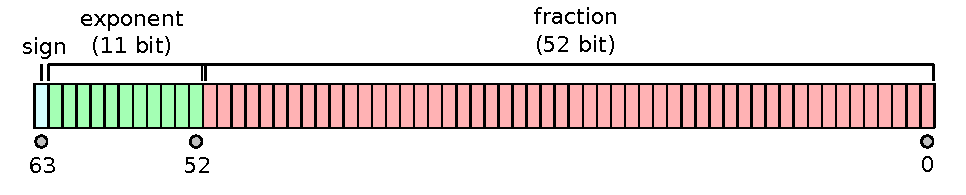
\includegraphics[width=1\textwidth]{pdf/double.pdf}
    \caption{Bitová reprezentace čísla v plovoucí řádce s dvojitou přesností dle IEE 754}
\end{figure}

Při ponechání prvních 12 bitů rozdělujeme interval čísel v plovoucí čárce na $2^{12}$ podintervalů.
Samotný výpočet podintervalu, do kterého zpracovávané číslo patří, je tedy realizovaný pomocí bitového posunu o 52 bitů doprava.

Dalším důsledkem bitové reprezentace čísel typu \texttt{double} je to, že pokud budeme ponechávat více než prvních 12 bitů (tedy když budeme ponechávat i bity mantisy), porovnávání dvou takových čísel zústane stále stejné.
Pomocí počtu bitů, které budeme posouvat, lze tedy jednoduše tedy konfigurovat počet podintervalů.

V případě, že by se v nějakém podintervalu i tak vyskytovalo příliš mnoho unikátních čísel, a nebylo by možné ho dále zpracovávat, je možné ponechávat dalších $n$ bitů následujících po bitech, které jsme ponechali při původním sestrojování histogramu, čímž podinterval rozdělíme na další podintervaly.

Rozdělování čísel do podintervalů pomocí bitového posunu poskytuje rychlý a jednoduchý způsob, jak rozdělovat čísla typu \texttt{double} do podintervalů, a tak efektivně sestavovat histogram i pro soubory, které se nevejdou do operační paměti.

\subsection{Paralelizace vyhledání percentilu}\label{parallel-bucketing}
Jelikož postup pro vyhledání percentilu v souboru uvedený v sekci \ref{bucketing} je velmi jednoduchý a výpočetně nenáročný, tak se zdá, že hlavním faktorem, který bude ovlivňovat dobu vyhledávání, bude rychlost čtení ze souboru (tedy přístup k IO).
Důsledkem toho je tedy efektivní paralelizace tohoto výpočtu složitá, jelikož čas strávený čekáním na IO je násobně větší než čas strávený sestavováním histogramu a jeho zpracováním za účelem vyhledání percentilu.

Jedním ze způsobů, jak provést paralelní vyhledávání percentilu, je takový způsob, kdy jedno vlákno čte ze souboru, a pomocí kruhového bufferu předává načtená data (čísla) dalším vláknům, která je zpracovávají. Výsledky výpočtů pak ukládají pomocí řízeného přístupu do chráněné paměti histogramu tak, aby nedošlo ke konfliktům. 
Další variantou tohoto způsobu, když zvolíme správnou velikost podintervalů, je způsob, kdy si každé vlákno sestavuje svůj vlastní histogram, a po přečtení celého souboru jsou histogramy vláken zkombinovány do jednoho hlavním vláknem, přičemž tato varianta je náročnější na velikost používaného paměťového prostoru výměnou za teoreticky rychlejší dobu vyhledávání z důvodu nepřítomnosti synchronizace při přístupů do sdílené paměti histogramu.

\begin{figure}[!ht]
    \centering 
    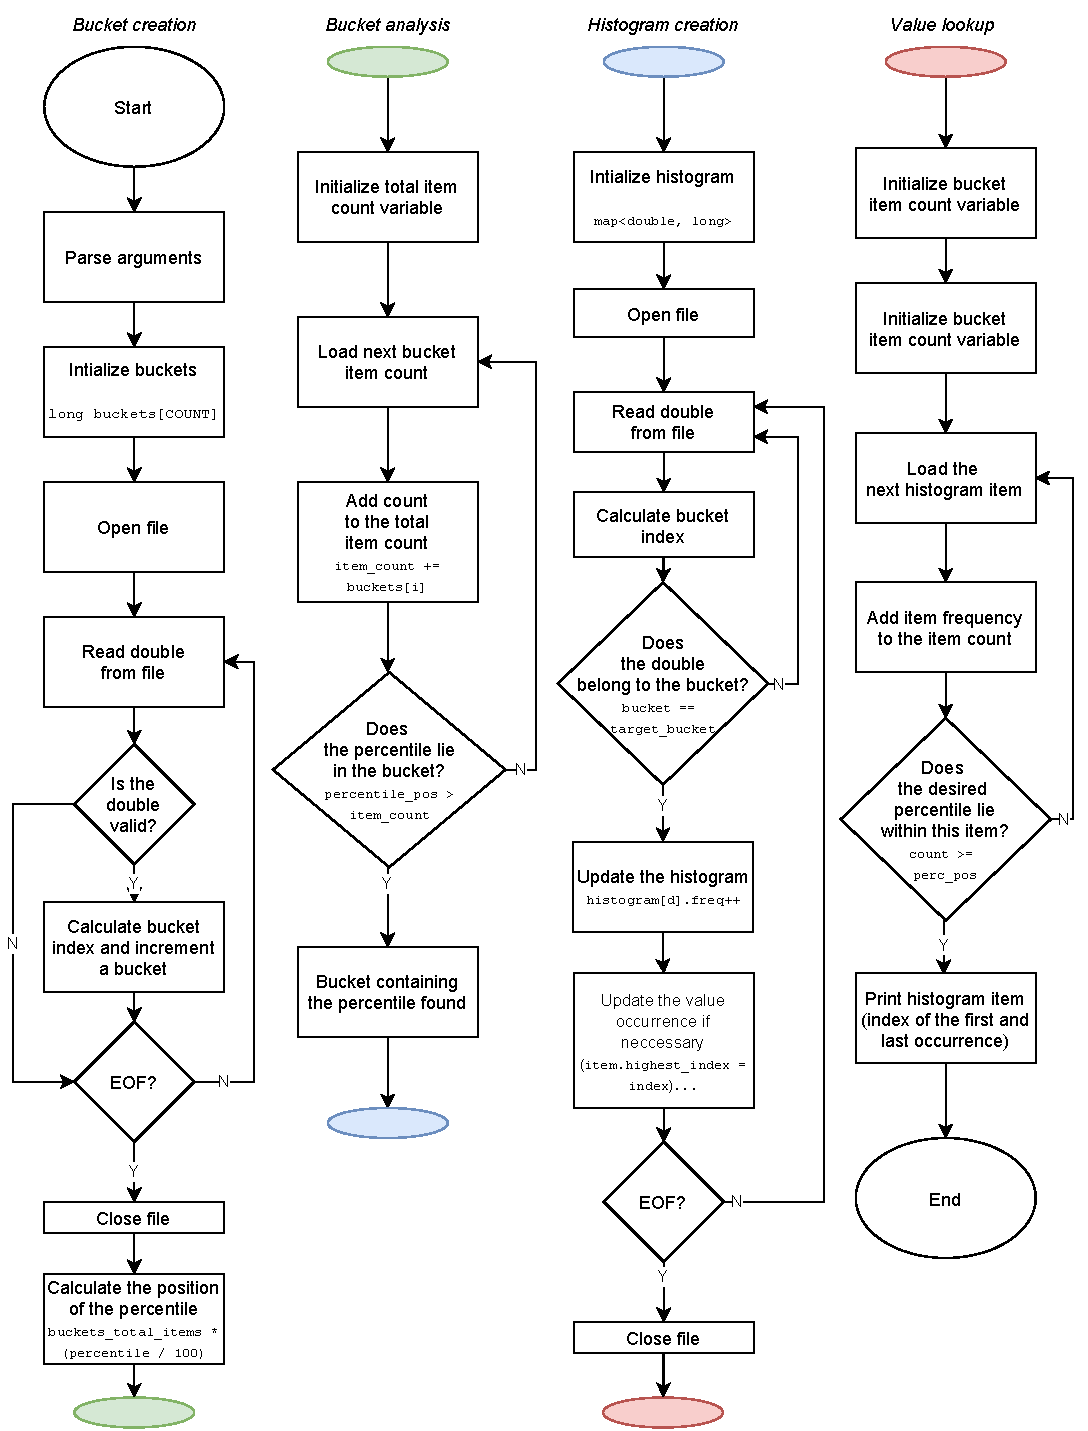
\includegraphics[width=1.038125\textwidth]{pdf/cfd.pdf}
    \caption{Diagram typu control-flow znázorňující zjednodušený postup používaný při vyhledávání percentilu v souboru s omezenou operační pamětí}
\end{figure}


\section{Popis implementace}

K vyhledávání percentilů v souborech byl zvolen postup popsaný v sekci \ref{bucketing} nakonfigurovaný tak, aby bylo během sestavování histogramu ponecháváno prvních \bucketingparamone~bitů čísla.
Pokud by se v podintervalu, ve kterém se nachází percentil, nacházelo příliš mnoho unikátních čísel, tak by se znovu spustilo sestavování histogramu, aby se počet unikátních čísel redukoval. 
Podinterval, ve kterém se nachází percentil, by se dělil na další podintervaly tak, že by se po původních \bucketingparamone~bitech ponechávalo i dalších \bucketingparamtwo~bitů. 
V každém podintervalu by tak mohlo být maximálně $2^{\bucketingparamthree}$~unikátních čísel.

\subsection{Sériová implementace}
Sériová implementace, při které probíhá výpočet jen na jednom vlákně, je velmi jednoduchá, a nachází se ve zdrojovém souboru \texttt{serial\_bucketing.cpp}.

%, kde jsou definovány dvě hlavní funkce: \texttt{create\_buckets\_serial} a \texttt{create\_buckets\_serial}.

Funkce \texttt{create\_buckets\_serial} sestavuje histogram z čísel nacházejících se ve vstupním souboru.
Velikost histogramu je daná počtem bitů, které jsou z každého načteného čísla ponechávány.

Po sestavení histogramu se vypočítá podinterval, ve kterém se percentil nachází, a přesná pozice relativní vůči seřazeným číslům nacházejících se v souboru. 

Poté se ve funkci \texttt{find\_percentile\_value\_serial} znovu čte celý vstupní soubor, ale zpracovávají se pouze čísla, která patří do výsledného podintervalu.

Výskyt každého zpracovávaného čísla je zaznamenáván do dalšího histogramu (již implementován pomocí datové struktury tabulka). 
Dále se také pro každé číslo zaznamenává jeho první a poslední výskyt v souboru.

Pokud by během druhého čtení souboru bylo načteno příliš mnoho unikátních čísel, a histogram s konkrétními čísly by se nevešel do omezené paměti, přistoupí se k rozdělení podintervalu na další podintervaly tak, jak je to popsáno v sekci \ref{bucketing}.

Nakonec, po zpracování celého souboru, je z histogramu, dle předtím vypočítané pozice, vybráno konkrétní číslo (včetně jeho výskytů), které je považováno za hledaný percentil.

Díky výpočtu percentilu pomocí bitového posunu a následné aktualizaci histogramu pomocí $O(1)$ operace (zápis dle indexu do \texttt{std::vector}) je sériová implementace velmi rychlá.

\subsection{Vícevláknová implementace}
Tato implementace využívá konstrukce \texttt{flow\_graph} z knihovny Intel Threading Building Blocks\footnote{\url{https://www.intel.com/content/www/us/en/developer/tools/oneapi/onetbb.html}} k paralelizaci výpočtu histogramu vycházejícího z algoritmu popsaném v sekci \ref{bucketing}.

První uzel grafu je typu \texttt{tbb::input\_node} a čte data ze vstupního souboru, která rovnou předává následujícím uzlům typu \texttt{tbb::function\_node} ke zpracování.
Každý tento uzel, jakmile obdrží data, je postupně zpracovává, ignoruje čísla, která dle zadání nejsou považována za validní, vypočítává podinterval pro vyfiltrovaná čísla a aktualizuje histogram. 

Každé vlákno, které zpracovává vstupní data, si vede vlastní histogram, aby nebylo třeba chránit přístup ke sdílené paměti.
Po zpracování celého souboru hlavní vlákno sloučí histogramy jednotlivých vláken do jednoho výsledného.

\begin{figure}[!ht]
    \centering 
    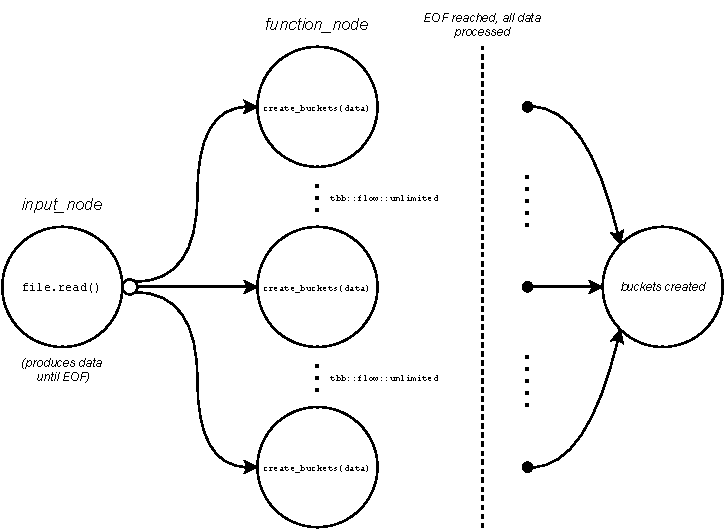
\includegraphics[width=1.0\textwidth]{pdf/create-buckets-tbb.pdf}
    \caption{Diagram popisující definici precedenčního grafu sestavení histogramu pomocí knihovny TBB}
\end{figure}

Po sestavení úvodního histogramu následuje sériový výpočet podintervalu, ve kterém se nachází hledaný percentil, a přesná pozice relativní vůči seřazeným číslům nacházejících se v souboru.

Nakonec se znovu zahájí paralelní výpočet, velmi podobný výpočtu popsanému v předchozích odstavcích, avšak s tím rozdílem, že se zpracovávají pouze ta čísla ze vstupního souboru, která patří do podintervalu ve kterém se nachází hledaný percentil.
Ke každému zpracovávanému číslu se vede záznam typu \texttt{bucket\_item}, který obsahuje informaci o hodnotě čísla, počtu výskytů čísla, jeho prvním a posledním výskytu v souboru.

Záznamy typu \texttt{bucket\_item} jsou jednotlivými uzly vkládány do sdílené tabulky, která je implementována pomocí typu \texttt{concurrent\_hash\_map}\footnote{\url{https://docs.oneapi.io/versions/latest/onetbb/tbb_userguide/concurrent_hash_map.html}} z jmenného prostoru knihovny TBB.
Tato tabulka, speciálně navržená pro využití v paralelních výpočtech, umožňuje bezpečný přístup k jejím hodnotám tak, aby nedošlo k nebezpečnému souběhu, kdy by k jedné hodnotě přistupovalo více vláken najednou.
Každý dotaz do tabulky dle klíče vrací hodnotu typu \texttt{accessor}, která, dokud není smazána, zabraňuje ostatním vláknům k chráněné hodnotě přistupovat.

Po druhém zpracování souboru, kdy je již sestavený histogram s konkrétními čísly nacházejícími se v souboru, se obdobně, jako v sériovém výpočtu, vyhledá percentil včetně jeho prvního a posledního výskytu, který je považován za výsledek.

\subsection{Implementace výpočtu s využitím OpenCL}
Jak již bylo zmíněno v sekci \ref{parallel-bucketing}, dosáhnout efektivní paralelizace navrženého výpočtu, která by byla výrazně rychlejší než sériové řešení, není jednoduché.

V rámci této semestrální práce však byl implementován postup, který využívá OpenCL k paralelizaci sestavování úvodního histogramu.
Hlavní vlákno načítá bloky čísel ze souboru (větší bloky než u ostatních předtím popsaných postupů za účelem redukce počtu nutných volání OpenCL zařízení),  které následně předává OpenCL zařízení, jež pro každé číslo zjistí, jestli se jedná o validní číslo dle zadání, pomocí bitového posunu spočítá do jakého podintervalu patří a aktualizuje histogram. 

\begin{table}[!ht]
    \begin{center}
        \begin{tabular}{ | m{6.5em} | m{1.5cm}| m{1.5cm} | m{1.5cm} | m{1.5cm} | } 
             \hline
             vstupní čísla & \texttt{double} & \texttt{double} & ... & \texttt{double} \\ 

             \hline
              po zpracování &  14573 & 14958 & ... & 1209 \\  

             \hline
        \end{tabular}
    \end{center}
    \caption{\label{tab:opencl-bucket-computation}Znázornění hromadného výpočtu podintervalů, do kterých zpracovávaná čísla patří.}
\end{table}

Hlavní vlákno nakonec načte z OpenCL zařízení sestavený histogram, zpracuje ho, a vypočte v jakém podintervalu se nachází hledaný percentil a jaká je jeho přesná pozice relativní vůči seřazeným číslům nacházejících se v souboru.

Poté hlavní vlákno začne vytvářet histogram již s konkrétními čísly. OpenCL zařízení se již nepoužívá, jelikož se jeho použití zde jeví jako neefektivní.

Během vývoje byl implementován výpočet, který v této fázi využíval OpenCL zařízení pouze k výpočtu podintervalů, do kterých zpracovávaná čísla patří, a následně byly podintervaly zpracovány hlavním vláknem, jež sestavovalo histogram s konkrétními čísly.
Tento výpočet byl však v porovnání se sériovým zpracování velmi pomalý, a tak nakonec nebyl použit.

Nakonec se po sestavení histogramu hlavním vláknem vyhledá v histogramu daný percentil dle pozice, která byla předtím vypočítána.
Tento percentil je pak považován za výsledek.

\subsection{Naivní implementace}
Za zmínku také stojí naivní implementace, která implementuje triviální algoritmus bez jakýchkoliv omezení na operační paměť, aby bylo možné porovnat, zdali ostatní implementace poskytují správné výsledky.

Tato implementace se nachází v souboru \texttt{naive.cpp}.

\section{Měření výkonnosti vytvořeného programu}

\subsection{Konfigurace testovacího prostředí}
Všechny testy byly prováděny na počítači s následujícím hardware:

\begin{itemize}
    \item \textbf{CPU} -- AMD Ryzen 5 1600 @ 3.2GHz, 6C / 12T, 16MB L3 cache, 14nm 
    \item \textbf{RAM} -- Crucial Ballistix Sport LT, 16GB (2x8GB) DDR4 2400 CL16
    \item \textbf{GPU} -- AMD RX480 @ 1208MHz, 4GB GDDR5 VRAM @ 7000 MHz
    \item \textbf{úložiště} -- Samsung 970 EVO 1TB, PCIe 3.0 4x NVMe, TLC, 3400 MB/s read, write 2500 MB/s
\end{itemize}

Výše zmíněná grafická karta vystupuje je dostupná pro výpočet v OpenCL pod názvem \textit{Ellesmere}.

Pro překlad zdrojových kódů byly použity překladače \texttt{g++} a \texttt{gcc} ve verzi 9.3.0 na operačním systému Ubuntu 20.04.3 LTS (Linux 5.4.0).

Překlad byl prováděn v režimu \texttt{release}.  

Některá měření byla prováděna na souboru \texttt{ubuntu-21.04-desktop-amd64.iso} (sha1: \texttt{34409f0432bd67fc12ad7b4aed6348da77b292fb}) o velikosti 2.7GiB. Tento soubor je dostupný na oficiálních stránkách operačního systému Ubuntu.

Jako nástroj pro měření byl zvolen program \texttt{time} běžně dostupný v Ubuntu OS.

\subsection{Výsledky měření}

V rámci měření byl program spuštěn čtyřikrát pro každé dostupné zařízení na soubor obsahující obraz Ubuntu OS. Hledaný byl percentil 50.
Časy běhů jsou zaznamenány v následující tabulce: 

\begin{table}[!ht]
    \begin{center}
        \begin{tabular}{ | m{6.5em} || m{1.5cm}| m{1.5cm} | m{1.5cm} | m{1.5cm} || m{1.7cm} |} 
             \hline
             Zařízení & 1. & 2. & 3. & 4. & Průměr[s] \\ 

             \hline
             \hline
              SINGLE &  4.197 & 4.308 & 4.195 & 4.257 & 4.239 \\  
              SMP & 5.486 & 5.466 & 5.496 & 5.535 & 5.495 \\
              Ellesmere & 3.294 & 3.069 & 3.374 & 3.105 & 3.211 \\

             \hline
        \end{tabular}
    \end{center}
    \caption{Časy běhů programu při zpracování souboru s obrazem Ubuntu OS.}
\end{table}

Z naměřených dat lze spočítat pro oba paralelní výpočty urychlení oproti sériové verzi dle následujícího vzorce:

\begin{equation}
    \begin{split}
    S = \frac{T_s}{T_p} \\ 
    \end{split}
\end{equation}

přičemž $T_s$ je čas běhu sériového výpočtu a $T_p$ čas běhu paralelního. 
Po dosazení naměřených hodnot do vzorce získáváme urychlení $0.771$ pro paralelní výpočet pomocí zařízení SMP, zatímco pro paralelní výpočet pomocí zařízení OpenCL (\textit{Ellesmere}) získáváme urychlení $1.32.$

Časy běhů programů pro percentil 50 a soubory různých velikostí obsahující náhodná data jsou zaznamenány v následujícím grafu:
\\
\\
\begin{figure}[!ht]
    \centering
    \begin{tikzpicture}
    \begin{axis}[
        width=\textwidth,
        ybar=.05cm,
        xlabel={Soubor},
        ylabel={Průměrný čas [s]},
    minor y tick num=2,
        ytick={0,1,2,3,4,5,6,7,8,9,10},
        bar width = 4pt,
        legend style={at={(0.45,0.9)},anchor=west},
        symbolic x coords={100MiB,200MiB,500MiB,1000MiB,2500MiB,5000MiB},
        xtick=data]
        \addplot coordinates {
            (100MiB,0.192)
            (200MiB,0.371)
            (500MiB,0.924)
            (1000MiB,1.894)
            (2500MiB,4.67)
            (5000MiB,9.014)
        };

        \addplot coordinates {
            (100MiB,0.248)
            (200MiB,0.458)
            (500MiB,1.074)
            (1000MiB,2.122)
            (2500MiB,5.16)
            (5000MiB,10.24)
        };

        \addplot coordinates {
            (100MiB,0.434)
            (200MiB,0.544)
            (500MiB,0.936)
            (1000MiB,1.614)
            (2500MiB,3.082)
            (5000MiB,5.814)
        };


        \legend {SINGLE, SMP, OpenCL};

    \end{axis}
    \end{tikzpicture}
    \caption{Graf zobrazující data naměřená při spouštění programu pro soubory o různých velikostech.}
\end{figure}

\newpage
Při získávání průměrných časů běhu programu pro náhodné soubory (generovány čtením z \texttt{/dev/urandom}) byl program spuštěn vždy pětkrát pomocí speciálního bash skriptu:

\begin{lstlisting}[language=bash,caption={Bash skript pro spuštění vytvořeného programu pro různé soubory a pro všechna dostupná zařízení.},captionpos=b, label={lst:benchmark-script}]
(
    for file in 100MiB 200MiB 500MiB 1000MiB 2500MiB 5000MiB
    do
        echo $file:
        echo "---------------"
        for device in SINGLE SMP Ellesmere
        do 
            echo $device:
            (/usr/bin/time -v ./pprsolver ../data/$file.bin 50 $device) 2>&1 | grep -E "Maximum resident set size|Elapsed|e) page faults"
        done 
    done
) | tee benchmark_result
\end{lstlisting}

\section{Uživatelská příručka}
\subsection{Sestavení}
Program lze sestavit buď pomocí Microsoft Visual Studio IDE po nahrání hlavičkových a zdrojových souborů do řešení nebo pomocí použití nástroje CMake: 

\begin{lstlisting}
cd src
cmake .
cmake --build . --target pprsolver
\end{lstlisting}

Po použití nástroje CMake vznikne v pracovním adresáři spustitelný program \texttt{pprsolver}.

\subsection{Použití}
Program vyžaduje při použití následující argumenty:

\begin{enumerate}
    \item cesta k souboru ke zpracování,
    \item hledaný percentil (číslo z rozsahu 1 až 100 včetně),
    \item a zařízení, které se má použít pro vyhledání percentilu (\texttt{SINGLE} -- jednovláknový výpočet, \texttt{SMP} -- vícevláknový výpočeta nebo název dostupného OpenCL zařízení).
\end{enumerate}

Ukázka spuštění programu pro obraz Ubuntu OS a hledaný percentil 50 při použití jednovláknového výpočtu:
\begin{lstlisting}
./pprsolver ubuntu-21.04-desktop-amd64.iso 50 SINGLE
\end{lstlisting}

\section{Závěr}

V rámci této semestrální práce byl vytvořen program napsaný v jazyce C++ 17, který umožňuje vyhledat percentil v libovolně velkém souboru i v případech, kdy je zpracovávaný soubor násobně větší než operační paměť dostupná programu.
Před spuštěním programu lze vybrat zdali má být výpočet sériový či paralelní.

Všechny tři implementované výpočty vycházejí z navrženého algoritmu, přičemž došlo jen k minimálním úpravám algoritmu oproti jeho původnímu návrhu.

Paralelní výpočet je implementován pomocí knihovny Intel Threading Building Blocks, a využívá konstrukce \texttt{tbb::flow\_graph}.

Druhý paralelní výpočet je implementován pomocí OpenCL, kdy je na OpenCL zařízení sestavován úvodní histogram.

Jelikož je navržený algoritmus pro vyhledávání percentilu v souboru velmi efektivní, tak jednotlivé paralelizace algoritmu nedosahují žádného nebo jen malého urychlení. 
Omezujícím faktorem pro urychlení pomocí paralelizace je také to, že velkou část času výpočtu se čeká na IO, kde nám paralelizace příliš nepomůže.

V případě paralelizace pomocí knihovny TBB byl tento výpočet rychlejší než jednovláknový výpočet pouze v případě, když nebyl program sestavován v režimu \texttt{release}.
Hlavním důvodem, proč je tato paralelizace pomalá, je to, že v jednotlivých vláknech nedochází k náročným výpočtům.
Dodatečná synchronizace mezi vlákny pak způsobuje, že oproti sériovému výpočtu dojde ke zpomalení.

Z výsledků měření lze pozorovat, že sestavování histogramu na OpenCL zařízení je dostatečně efektivní a přináší tak zrychlení oproti sériovému výpočtu.
Jedním z důvodů viditelného zrychlení je fakt, že data ze vstupního souboru jsou v případě výpočtu pomocí OpenCL zařízení čtena po větších blocích, než u ostatních výpočtů, a tak je dobře využita paralelizace výpočtu pro jednotlivá čísla a redukuje se i počet volání čtení ze souboru.

Pokud bychom chtěli dosáhnout lepších výsledků paralelizace, bylo by třeba se pokusit navrnout jiný algoritmus pro vyhledání percentilu, který by šel lépe paralelizovat.
Osobně si však myslím, že navržený algoritmus, který čerpá hlavně z využití bitového posunu, je dostatečně dobrý.


\end{document}

